\documentclass[10pt,twocolumn]{article}
\usepackage[utf8]{inputenc}
\usepackage[spanish,es-nodecimaldot]{babel}
\usepackage[letterpaper,top=1.25cm,bottom=1.25cm,left=1.3cm,right=1.3cm]{geometry}
\usepackage{amsmath,amssymb,amsfonts}
\usepackage{lmodern}
\usepackage{graphicx}
\usepackage{booktabs}
\usepackage{microtype}
\usepackage{titlesec}
\usepackage{caption}
\usepackage{hyperref}

\hypersetup{colorlinks=true,linkcolor=black,citecolor=black,urlcolor=blue}

% Ajustes ultra-compactos para calzar exactamente en 2 páginas
\titleformat{\section}{\bfseries\normalsize}{\thesection.}{0.3em}{}
\titlespacing*{\section}{0pt}{3pt}{1pt}
\titleformat{\subsection}{\bfseries\small}{\thesubsection.}{0.3em}{}
\titlespacing*{\subsection}{0pt}{2pt}{1pt}

\captionsetup{font=footnotesize,labelfont=bf,skip=2pt}

\setlength{\columnsep}{13pt}
\setlength{\parindent}{8pt}
\setlength{\parskip}{0pt}
\setlength{\abovedisplayskip}{2.5pt}
\setlength{\belowdisplayskip}{2.5pt}
\setlength{\abovedisplayshortskip}{1.5pt}
\setlength{\belowdisplayshortskip}{1.5pt}
\setlength{\jot}{1.5pt}

\begin{document}

\twocolumn[
  \begin{@twocolumnfalse}
    {\noindent\Large\textbf{Modelos de Espacio de Estados y el Filtro de Kalman:}\\[1.5pt]
    \textbf{Formulación Canónica, Dinámica Recursiva y Diagnóstico}\par}
    \vspace{2pt}
    {\noindent\normalsize\textbf{Jorge, Mattias y Miguel Ángel Camargo Mora}\par}
    \vspace{1.5pt}
    {\noindent\footnotesize\textit{Series de Tiempo $\cdot$ Ciencia de Datos, Universidad Externado de Colombia $\cdot$ Informe ejecutivo, noviembre de 2026}\par}
    \vspace{3pt}
    {\noindent\footnotesize\textbf{Resumen.} Los modelos clásicos ARMA/ARIMA suponen que las variables de interés se observan directamente sin error de medición. En macroeconomía y finanzas, las variables fundamentales (PIB potencial, tasa natural de interés, brechas de política y expectativas) son inobservables (latentes) y las series registradas contienen ruido y retrasos. El marco de \textbf{Espacio de Estados} desacopla la física del estado oculto de la ecuación del sensor observable. El \textbf{Filtro de Kalman} proporciona el estimador recursivo óptimo de mínima varianza que actualiza las expectativas en tiempo real ante la llegada de cada nuevo dato sin almacenar el pasado. Este informe expone la estructura matricial canónica, describe formalmente todas sus variables, detalla las tres fases del motor recursivo, formaliza las pruebas de diagnóstico y desarrolla un ejemplo numérico univariado completo con 5 observaciones.\par}
    \vspace{5pt}
  \end{@twocolumnfalse}
]

% Banner de la Figura 2 ubicado en el tope de la Página 2
\begin{figure*}[t]
\centering
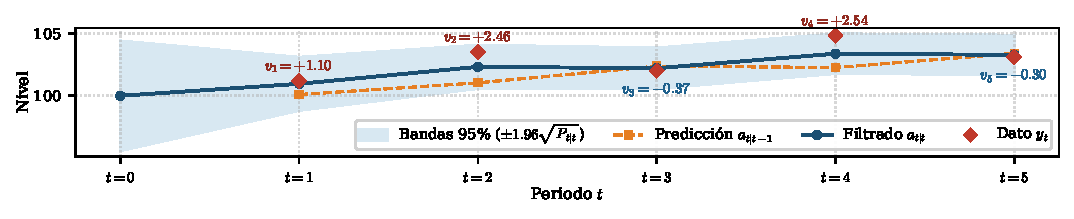
\includegraphics[width=\textwidth]{fig2_ejemplo.pdf}
\caption{Evolución dinámica del Filtro de Kalman en las 5 observaciones del ejemplo numérico. La predicción $a_{t|t-1}$ confronta la observación $y_t$ generando la innovación $v_t$; el estado filtrado $a_{t|t}$ actualiza la trayectoria reduciendo drásticamente la incertidumbre ($\pm 1.96\sqrt{P_{t|t}}$).}
\label{fig:ejemplo_banner}
\end{figure*}

\section{Motivación: variables latentes}

En econometría contemporánea, las variables de decisión casi nunca admiten registro contable directo. El marco de \textbf{componentes no observados} descompone una serie temporal observada $y_t$ en sus fuerzas generadoras fundamentales:
\begin{equation}
y_t = \mu_t + c_t + \gamma_t + \varepsilon_t, \quad \varepsilon_t \sim \text{WN}(0, \sigma_\varepsilon^2). \tag{1}
\end{equation}
donde $y_t \in \mathbb{R}$ es la serie empírica observada en el periodo $t$ (ej. PIB o índice de actividad), $\mu_t$ es la tendencia secular estocástica de largo plazo ($\mu_t = \mu_{t-1} + \beta_{t-1} + \eta_{\mu,t}$), $c_t$ es el ciclo económico oscilatorio transitorio, $\gamma_t$ es el componente estacional ligado al calendario, y $\varepsilon_t$ es el ruido blanco irregular de medición con varianza $\sigma_\varepsilon^2$. Dado que ninguno de estos componentes se observa de manera aislada, el objetivo consiste en extraer probabilísticamente el vector de estado oculto $\alpha_t$ a partir de la señal ruidosa $y_t$ (Figura 1).

\begin{center}
\vspace{1pt}
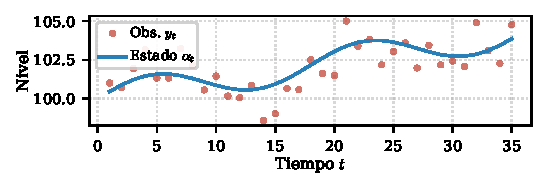
\includegraphics[width=\columnwidth]{fig1_latente.pdf}
\captionof{figure}{Señal observable ruidosa $y_t$ frente al estado latente subyacente $\alpha_t$. El espacio de estados separa la corriente real del error.}
\label{fig:latente}
\vspace{1pt}
\end{center}

\section{Representación de Espacio de Estados}

El sistema dinámico lineal se describe mediante dos ecuaciones matriciales acopladas (Harvey, 1989; Hamilton, 1994):

\noindent\textbf{1. Ecuación Canónica de Transición.} Rige la evolución física del vector de variables ocultas:
\begin{equation}
\alpha_t = T_t \alpha_{t-1} + c_t + R_t \eta_t, \quad \eta_t \sim \mathcal{N}(0, Q_t), \tag{2}
\end{equation}
donde $\alpha_t \in \mathbb{R}^{m \times 1}$ es el \textbf{vector de estado latente} en $t$ (reúne todas las variables no observadas del sistema), $T_t \in \mathbb{R}^{m \times m}$ es la \textbf{matriz de transición} que rige la persistencia intrínseca, $c_t \in \mathbb{R}^{m \times 1}$ es el \textbf{vector de deriva} determinística, $R_t \in \mathbb{R}^{m \times g}$ es la \textbf{matriz de selección de shocks}, $\eta_t \in \mathbb{R}^{g \times 1}$ es el \textbf{vector de perturbaciones del sistema} (shocks gaussianos no observables) y $Q_t \in \mathbb{R}^{g \times g}$ es su \textbf{matriz de covarianza}, que cuantifica la volatilidad de los shocks al estado.

\noindent\textbf{2. Ecuación Canónica de Medida.} Vincula el estado con las magnitudes observables:
\begin{equation}
y_t = Z_t \alpha_t + d_t + \varepsilon_t, \quad \varepsilon_t \sim \mathcal{N}(0, H_t), \tag{3}
\end{equation}
donde $y_t \in \mathbb{R}^{N \times 1}$ es el \textbf{vector observable} de $N$ series medidas, $Z_t \in \mathbb{R}^{N \times m}$ es la \textbf{matriz de medición} que proyecta los estados hacia los indicadores, $d_t \in \mathbb{R}^{N \times 1}$ es el vector de intercepto del sensor, $\varepsilon_t \in \mathbb{R}^{N \times 1}$ es el \textbf{error de medición} (ortogonal a $\eta_t$: $\mathbb{E}[\eta_t \varepsilon_\tau^\top] = 0$) y $H_t \in \mathbb{R}^{N \times N}$ es la \textbf{covarianza del ruido de medida}.

\noindent\textbf{Forma Compañera para AR($p$).} Para un ciclo con $p$ rezagos $c_t = \sum_{j=1}^p \phi_j c_{t-j} + \eta_t$, se apila el pasado en un vector aumentado preservando la propiedad markoviana de primer orden:
\begin{equation}
\begin{bmatrix} c_t \\ c_{t-1} \\ \vdots \\ c_{t-p+1} \end{bmatrix} = \begin{bmatrix} \phi_1 & \phi_2 & \cdots & \phi_p \\ 1 & 0 & \cdots & 0 \\ \vdots & \ddots & & \vdots \\ 0 & \cdots & 1 & 0 \end{bmatrix} \begin{bmatrix} c_{t-1} \\ c_{t-2} \\ \vdots \\ c_{t-p} \end{bmatrix} + \begin{bmatrix} 1 \\ 0 \\ \vdots \\ 0 \end{bmatrix} \eta_t. \tag{4}
\end{equation}
La fila superior contiene los parámetros autoregresivos $\{\phi_j\}$; la identidad desplazada $I_{p-1}$ almacena mecánicamente la memoria.

\noindent\textbf{Estabilidad y Ecuación de Lyapunov.} El sistema es estable si y solo si todos los autovalores cumplen $|\lambda_i(T)| < 1$. La covarianza incondicional $P_\infty = \text{Var}(\alpha_t)$ resuelve la ecuación discreta de Lyapunov:
\begin{equation}
P_\infty = T P_\infty T^\top + R Q R^\top \iff \text{vec}(P_\infty) = [I_{m^2} - (T \otimes T)]^{-1} \text{vec}(R Q R^\top), \tag{5}
\end{equation}
donde $\otimes$ es el producto de Kronecker. Esto proporciona la inicialización teórica exacta del filtro: $a_{0|0} = \mathbb{E}[\alpha_t]$ y $P_{0|0} = P_\infty$.

\section{El Motor Recursivo de Kalman}

El Filtro de Kalman (1960) opera como un algoritmo en tres fases:

\noindent\textbf{Fase 1: Predicción a priori ($t-1 \to t$).} Proyecta el estado y su dispersión antes de observar el periodo $t$:
\begin{align}
a_{t|t-1} &= T_t a_{t-1|t-1} + c_t, \tag{6} \\
P_{t|t-1} &= T_t P_{t-1|t-1} T_t^\top + R_t Q_t R_t^\top, \tag{7}
\end{align}
donde $a_{t|t-1} = \mathbb{E}[\alpha_t | \mathcal{Y}_{t-1}]$ es la mejor predicción lineal y $P_{t|t-1} = \text{Var}(\alpha_t | \mathcal{Y}_{t-1})$ su incertidumbre proyectada.

\noindent\textbf{Fase 2: Innovación y sorpresa ($y_t$).} Confronta la expectativa con la realidad empírica observada:
\begin{align}
v_t &= y_t - Z_t a_{t|t-1} - d_t, \tag{8} \\
F_t &= Z_t P_{t|t-1} Z_t^\top + H_t, \tag{9}
\end{align}
donde $v_t \in \mathbb{R}^N$ es la \textbf{innovación} (error de predicción) y $F_t \in \mathbb{R}^{N \times N}$ su matriz de covarianza.

\noindent\textbf{Fase 3: Actualización a posteriori (Forma de Joseph).} Pondera óptimamente la sorpresa para corregir el estado:
\begin{align}
K_t &= P_{t|t-1} Z_t^\top F_t^{-1}, \tag{10} \\
a_{t|t} &= a_{t|t-1} + K_t v_t, \tag{11} \\
P_{t|t} &= (I - K_t Z_t) P_{t|t-1} (I - K_t Z_t)^\top + K_t H_t K_t^\top. \tag{12}
\end{align}
La \textbf{Ganancia de Kalman} $K_t \in \mathbb{R}^{m \times N}$ optimiza la ponderación: si el ruido $H_t$ domina, $K_t \to 0$ y prima el modelo; si la señal es limpia, $K_t \to Z_t^{-1}$. La forma de Joseph (12) garantiza semidefinición positiva frente a cancelaciones numéricas.

\noindent\textbf{Datos Faltantes y Máxima Verosimilitud.} Si una variable es inobservable en $t$ ($\text{NaN}$), se elimina su fila en $y_t, Z_t$ y $H_t$. Si falta todo el vector, $a_{t|t} = a_{t|t-1}$ y $P_{t|t} = P_{t|t-1}$. Los hiperparámetros se estiman maximizando la log-verosimilitud por descomposición del error de predicción:
\begin{equation}
\ln \mathcal{L}(\theta) = -\frac{1}{2} \sum_{t=1}^T \left[ N \ln(2\pi) + \ln |F_t| + v_t^\top F_t^{-1} v_t \right]. \tag{13}
\end{equation}

\section{Diagnóstico, validación y robustez}

Si el modelo está correctamente especificado, las innovaciones estandarizadas $e_t = F_t^{-1/2} v_t$ deben cumplir $e_t \overset{\text{i.i.d.}}{\sim} \mathcal{N}(0, I_N)$. Para auditar esta propiedad se aplican tres contrastes:

\noindent\textbf{1. Ljung-Box (independencia):} $Q_{LB} = T(T+2) \sum_{k=1}^s \frac{r_k^2}{T-k} \sim \chi^2(s)$, con $r_k$ la autocorrelación de $e_t$. Si $p < 0.05$, se rechaza la ausencia de correlación (faltan rezagos en $T$).

\noindent\textbf{2. Jarque-Bera (normalidad):} $JB = \frac{T}{6} [ S^2 + \frac{(K-3)^2}{4} ] \sim \chi^2(2)$, con $S$ asimetría y $K$ curtosis. Detecta saltos o colas pesadas.

\noindent\textbf{3. Criterios AIC y BIC:} $\text{AIC} = -2\ln\mathcal{L} + 2k$ y $\text{BIC} = -2\ln\mathcal{L} + k\ln(T)$ para seleccionar el orden $p$ óptimo.

\noindent\textbf{Divergencia del Filtro.} Ocurre cuando $P_{t|t} \to 0$ por subestimar $Q$, anulando la ganancia ($K_t \to 0$) e ignorando los datos reales. Se mitiga mediante inflación de covarianza ($P_{t|t-1} = \lambda T P T^\top + Q$ con $\lambda > 1$) o estimadores robustos de Huber con umbral $c \approx 1.345$: $\rho(e) = \frac{1}{2} e^2$ si $|e| \le c$ y $c|e| - \frac{1}{2}c^2$ si $|e| > c$.

\section{Ejemplo numérico paso a paso (5 datos)}

Se implementa el motor sobre un modelo escalar ($m=N=1$) que rastrea un índice latente con parámetros:
$T = 0.98$, $c = 2.10$, $R = 1$, $Q = 0.50$, $Z = 1$, $H = 1.50$; condiciones iniciales $a_{0|0} = 100.0$ y $P_{0|0} = 5.0$. La secuencia observada es $y = [101.2, 103.5, 102.0, 104.8, 103.1]$.

\begin{table}[h]
\centering
\footnotesize
\caption{Iteraciones completas del Filtro de Kalman ($t=1$ a $5$).}
\begin{tabular}{@{}ccccccccc@{}}
\toprule
$t$ & $y_t$ & $a_{t|t-1}$ & $P_{t|t-1}$ & $v_t$ & $F_t$ & $K_t$ & $a_{t|t}$ & $P_{t|t}$ \\
\midrule
1 & 101.2 & 100.100 & 5.302 & +1.100 & 6.802 & 0.779 & 100.957 & 1.169 \\
2 & 103.5 & 101.038 & 1.623 & +2.462 & 3.123 & 0.520 & 102.317 & 0.780 \\
3 & 102.0 & 102.371 & 1.249 & -0.371 & 2.749 & 0.454 & 102.202 & 0.682 \\
4 & 104.8 & 102.258 & 1.155 & +2.542 & 2.655 & 0.435 & 103.364 & 0.653 \\
5 & 103.1 & 103.397 & 1.127 & -0.297 & 2.627 & 0.429 & 103.270 & 0.643 \\
\bottomrule
\end{tabular}
\label{tab:ejemplo}
\end{table}

\noindent\textbf{Cálculo analítico iterativo:}
En $t=1$, $a_{1|0} = 0.98(100) + 2.10 = 100.10$, $P_{1|0} = (0.98)^2(5) + 0.5 = 5.302$. Sorpresa $v_1 = 101.2 - 100.10 = +1.100$ ($F_1 = 6.802$). Con alta incertidumbre previa, la ganancia confía en el dato: $K_1 = 5.302/6.802 = 0.7794$, dando $a_{1|1} = 100.10 + 0.7794(1.10) = 100.957$ y reduciendo la varianza a $P_{1|1} = 1.169$. En $t=2$, $a_{2|1} = 101.038$, $P_{2|1} = 1.623$, $v_2 = +2.462$, $K_2 = 0.5196$, dando $a_{2|2} = 102.317$ y $P_{2|2} = 0.780$. En $t=3$, la sorpresa negativa $v_3 = -0.371$ corrige el estado hacia $a_{3|3} = 102.202$ con $K_3 = 0.4544$. En $t=4$ y $t=5$, el filtro procesa $v_4 = +2.542$ y $v_5 = -0.297$, alcanzando $a_{5|5} = 103.270$ y $P_{5|5} = 0.643$.

\begin{center}
\vspace{1pt}
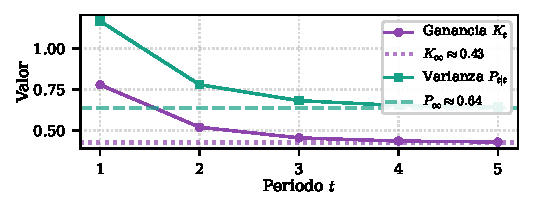
\includegraphics[width=\columnwidth]{fig3_convergencia.pdf}
\captionof{figure}{Convergencia monótona de la Ganancia $K_t$ y de la incertidumbre $P_{t|t}$ hacia el límite de Lyapunov ($P_\infty \approx 0.638, K_\infty \approx 0.426$).}
\label{fig:convergencia}
\vspace{1pt}
\end{center}

\section{Conclusiones}

\begin{enumerate}
    \setlength{\itemsep}{0pt}\setlength{\parskip}{0pt}
    \item \textbf{Aislamiento óptimo de señal y ruido:} El espacio de estados separa la dinámica oculta del error instrumental sin recurrir a diferenciaciones espurias.
    \item \textbf{Eficiencia recursiva:} El filtro actualiza condicionalmente usando solo la innovación presente $v_t$, optimizando memoria y cómputo.
    \item \textbf{Convergencia demostrada:} En solo 5 observaciones (Tabla 1 y Figuras 2 y 3), la incertidumbre $P_{t|t}$ y la ganancia $K_t$ alcanzan el equilibrio de Lyapunov.
    \item \textbf{Validación rigurosa:} La bondad de ajuste descansa en la blancura gaussiana de $e_t$ contrastada mediante Ljung-Box y Jarque-Bera.
\end{enumerate}

\begin{thebibliography}{9}
\footnotesize
\setlength{\itemsep}{0pt}\setlength{\parskip}{0pt}
\bibitem{kalman1960} Kálmán, R. E. (1960). A new approach to linear filtering and prediction problems. \textit{J. Basic Eng.}, 82(1), 35--45.
\bibitem{harvey1989} Harvey, A. C. (1989). \textit{Forecasting, Structural Time Series Models and the Kalman Filter}. Cambridge Univ. Press.
\bibitem{hamilton1994} Hamilton, J. D. (1994). \textit{Time Series Analysis}. Princeton Univ. Press.
\bibitem{durbin2012} Durbin, J. y Koopman, S. J. (2012). \textit{Time Series Analysis by State Space Methods}. Oxford Univ. Press.
\end{thebibliography}

\end{document}
